\section{Behavioral Composition Approaches}

In this section, we focus on approaches that deal with composition of behaviors. We categorize the state of art approaches into two groups. We begin by approaches that compose behavioral models. They specify the composition at language level, and then, they automate the composition of behavioral models (see Figure~\ref{fig:behacompomodel}). We finish this section by approaches that aim at compositing the behavioral semantics of languages into a new semantics.  

\begin{figure}
	\begin{center}
		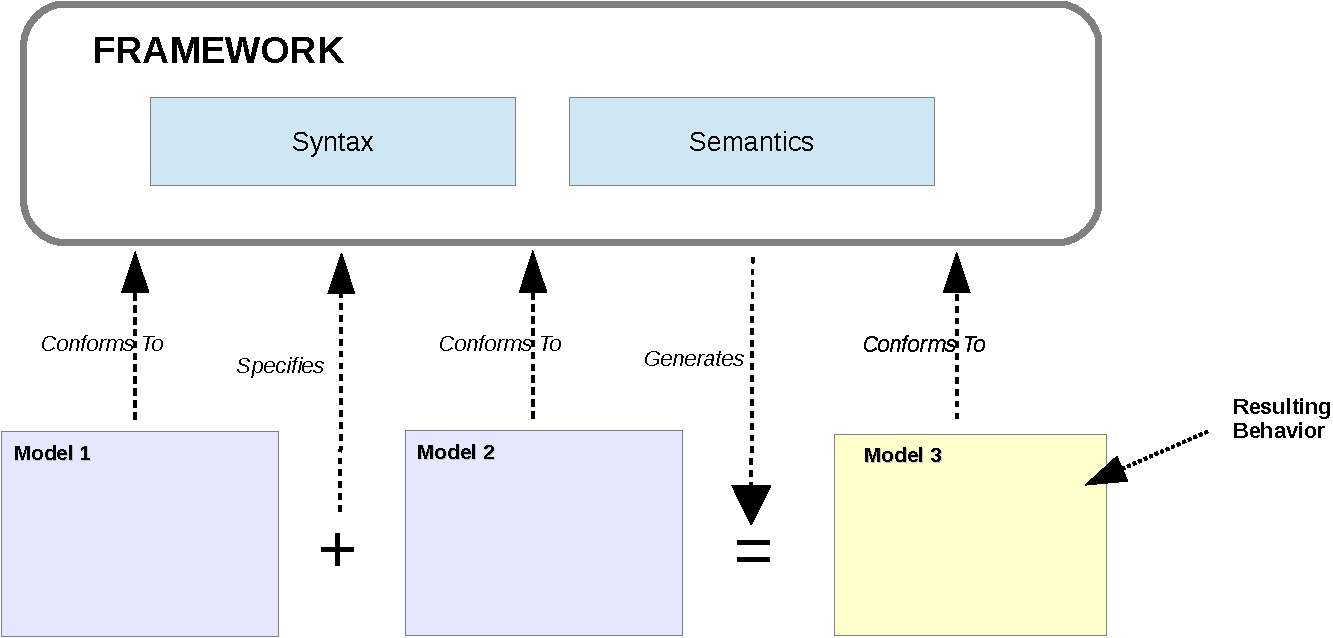
\includegraphics[width=.7\columnwidth]{background/figs/behacompomodel}
		\caption{Overview of Composition of Behavioral Models Approaches}
		\label{fig:behacompomodel}
	\end{center}
\end{figure}
	
\subsection{Composition of Behavioral Models}

In \cite{compostatechartsbib}, authors relay on statecharts to describe the behavior of models. Then, they propose an automatic approach to compose statecharts into a new statechar model. The resulting model represents the global behavior. The approach is based on a matching and a merging operator. The matching is used to produce correspondence relationships between states of two models. The matching can be \emph{static} and \emph{behavioral}. The static matching is based on a naming convention thus relying on the syntax of statechart. Conversely, the behavioral matching selects pair of states by relying on their behavioral semantics. The merging operator takes as input two models and a correspondence relation, and it generates a new model conforming to statecharts that represents the global emerging behavior. This approach is implemented in a tool named TReMer~\footnote{https://se.cs.toronto.edu/index.php/TReMer\%2B}. %A similar approach is presented in~\cite{compoclassdiagrambib}. However, in this approach, authors represents the behavior of models by using se   
		 
Aspect Oriented Modeling provides a different approach through the weaving of aspects that encapsulate behaviors~\cite{weavingbib}. Advices represent a new behavior that should replace the base behavior when it is matched by the pointcut. For instance, in AspectJ~\cite{AspectJoverview}, the aspects are used to extend Java and the advice is expressed in Java code. Similarly, RAM~\cite{rambib,composdbib} is an aspect oriented approach in which the behavior of aspects is described by using sequence diagrams. The approach proposes the composition of behavioral models by relying on the weaving of sequence diagrams.

The previous approaches specify how behavioral models can be composed into a new model that represents the resulting system behavior. In the next subsection, we overview approaches that specify how the behavioral semantics of languages can be composed into a new semantics.

\subsection{Composition of Language Behavioral Semantics}
To our knowledge, only Chen et al.~\cite{semanticsanchoring} propose to define the semantics of a language by composing other semantics. In this work, a \emph{Semantic Unit} (SU) is represented by a structure (\emph{Abstract Data Model}) and a behavioral semantics. The approach specifies the SU in the \emph{Abstract State Machine Language}\footnote{http://research.microsoft.com/en-us/projects/asml/} (Asml). This language is used to specify both the structure and the semantics of a SU. A given SU is associated to the Abstract Syntax (AS) of a language through a mapping. The mapping associates each element in the AS with an element in the Abstract Data Model of the SU. This approach  enables the system designer to compose two SU into a new one. For instance, in~\cite{composemanticanch}, authors define two SU named Finite State Machine (FSM) and Synchronize Data Flow (SDF), and then, they specify how the two SU can be composed into a new one called EFSM.  

\subsection{Discussion}
Composition of Behavioral Models approaches rely on a common semantics to describe the behavioral of models. Then, they automated the composition of behavioral models by relying on a set of rules at language level. In~\cite{semanticsanchoring}, authors also rely on a common semantics to describe the behavioral semantics of languages (\eg Asml) and a set of rules between semantics elements. However, these rules specify how the semantics of languages can be composed into a new semantics. In a complex system, where heterogeneous languages may be used, a unified language could be hard to handle thus limiting the reusability.
In the following section, we study approaches that propose to coordinate behavioral models by specifying a \emph{model of coordination}.